%\document{article}
\documentclass[UTF8]{ctexart}
\usepackage{listings} 
\usepackage{amsmath}
\usepackage{graphicx}
\usepackage{fancyhdr}
\usepackage{float}

\title{ALU}
\author{朱河勤   PB16030899}
\pagestyle{fancy}
\lhead{朱河勤   PB16030899}
\chead{ALU}
\rhead{2018/3/29}
\begin{document}
\maketitle
\tableofcontents

\section{实验目的}

\paragraph{1}熟练掌握ALU的构成

\paragraph{2}掌握ALU的原理

\section{实验要求}
\paragraph{*}用模块化设计,实现斐波那契数列
\paragraph{*}实现ALU的计算功能,包括add,sub,and, or,
xor,ornot,nop

\section{实验平台}
gtkwave+iverilog



\section{实验分析}
\paragraph{1}由于有op来选择计算操作符,所以可以用case语句
\paragraph{2}为了输出所有的斐波那契数列值,需要实例化多个alu模块

\section{实验结果}
成功满足要求,这是仿真结果


\begin{figure}[H]
  \centering
  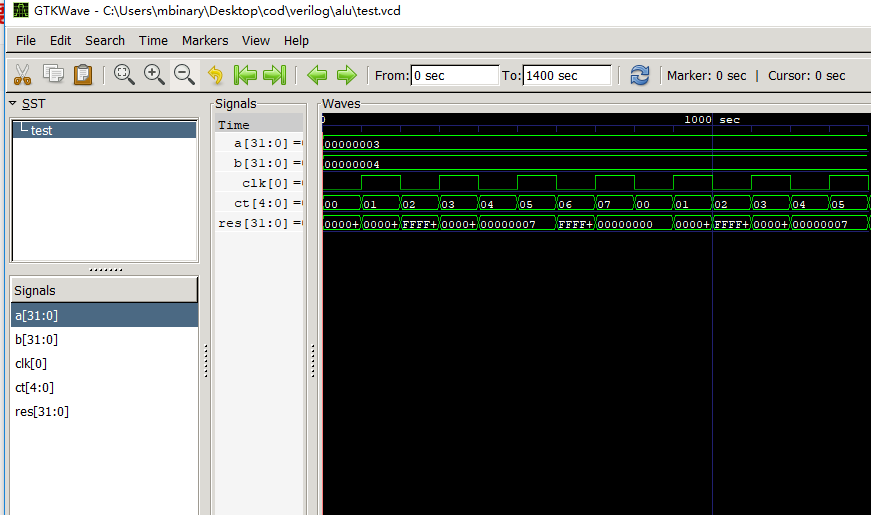
\includegraphics[width=1\textwidth]{test.png}
\end{figure}




\section{源代码}

\begin{verbatim}

//alu
`ifndef  _alu
`define _alu


module alu(
		input signed  [31:0] alu_a,
		input signed  [31:0] alu_b,
		input 		  [4:0] alu_op,
		output        [31:0] alu_out);
		
		reg [31:0] res;
		assign alu_out = res;
		
		always@(*)
		begin
			case(alu_op)
			0:res=0;             // nop
			1:res=alu_a+alu_b;   // add
			2:res=alu_a-alu_b;  //  sub
			3:res=alu_a&alu_b;  //  and
			4:res=alu_a|alu_b;   //  or
			5:res=alu_a ^ alu_b;  //  xor 
			6:res= ~(alu_a|alu_b); //   ornot
			default:res=0;       // nop
			endcase
		end
endmodule
`endif



//top
module top();

	reg [31:0] alu_a=2;
	reg [31:0] alu_b=2;
	reg [31:0] n1,n2,n3,n4;
	alu a1(alu_a,alu_b,1,n1);
	alu a2(n1,alu_b,1,n2);
	alu a3(n1,n2,1,n3);
	alu a4(n2,n3,1,n4);
	
endmodule


//testbench
module test();

initial begin
    $dumpfile("test.vcd");
    $dumpvars(1,test);
    end
    
    reg clk=0;
    reg [4:0] ct=0;

    
    reg [31:0]    a=3,b=4;
    wire  [31:0] res;
    alu i(a,b,ct,res);
    always #100 begin
        clk = ~clk;
        if(ct==7)ct=0;
        else ct =ct+1;
    end
    
initial #1400 
    $finish;	
endmodule


\end{verbatim}

\end{document}